
%(BEGIN_QUESTION)
% Copyright 2011, Tony R. Kuphaldt, released under the Creative Commons Attribution License (v 1.0)
% This means you may do almost anything with this work of mine, so long as you give me proper credit

Beregn følgende parametere i dette balanserte 3-fase elektriske kraftsystemet:

$$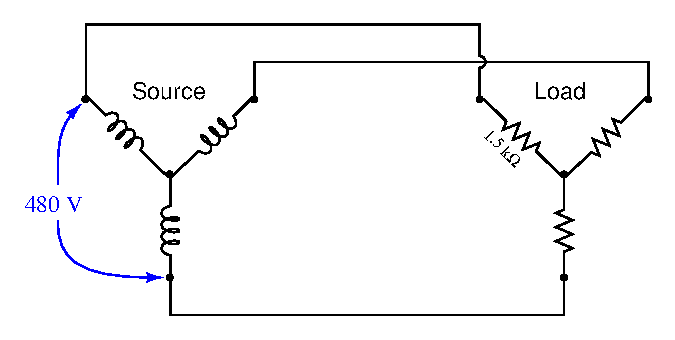
\includegraphics[width=15.5cm]{i00915x01.eps}$$

\begin{itemize}
%\item{} $V_{line} =$
%\vskip 10pt
\item{} $I_{line} =$
\vskip 10pt
%\item{} $V_{phase(source)} =$
%\vskip 10pt
%\item{} $I_{phase(source)} =$
%\vskip 10pt
%\item{} $V_{phase(load)} =$
%\vskip 10pt
\item{} $I_{phase(load)} =$
\end{itemize}

\underbar{file i00915}
%(END_QUESTION)





%(BEGIN_ANSWER)

\begin{itemize}
\item{} $I_{line} =$ 0.1848 ampere
\vskip 10pt
\item{} $I_{phase(load)} =$ 0.1848 ampere
\end{itemize}


%(END_ANSWER)





%(BEGIN_NOTES)

{\bf Denne oppgaven er ment kun for eksamen, ikke for arbeidsark!}.

%(END_NOTES)

